\begin{figure*}[!htbp]
    \centering
    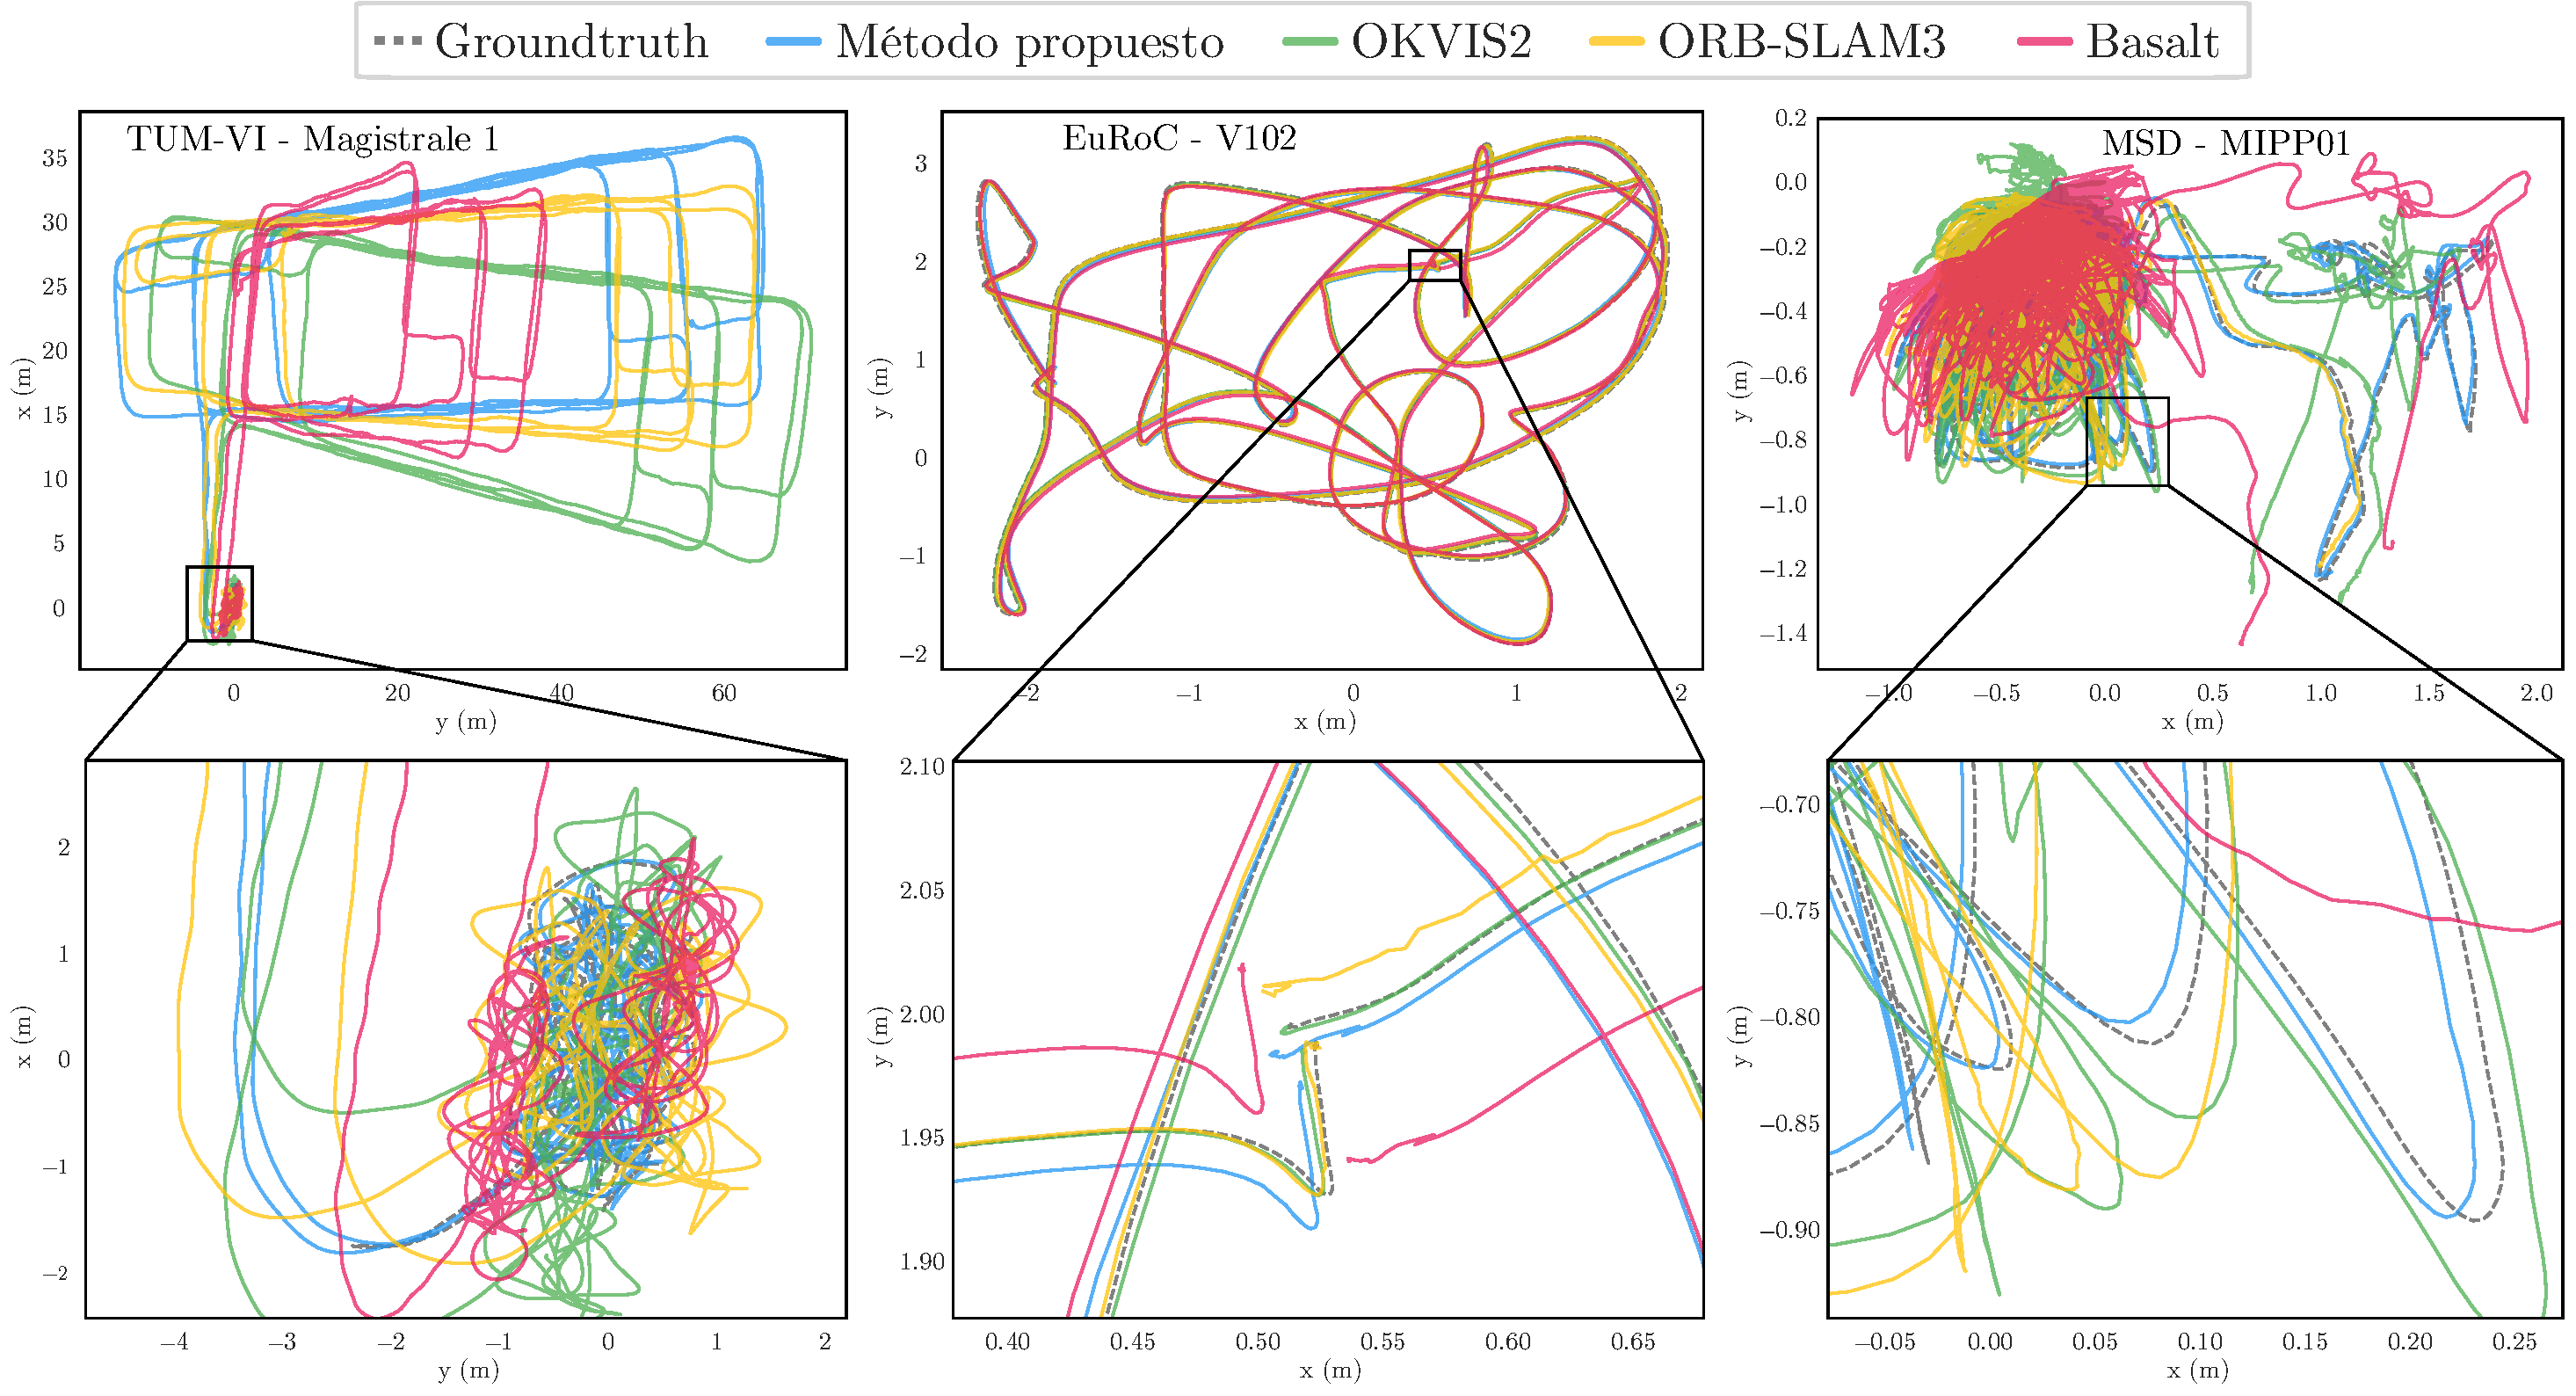
\includegraphics[width=1\linewidth]{images/trajectories.pdf}
    \caption{Ejemplos de trayectorias para secuencias de distintos datasets, con ampliaciones en partes que resultan de interés. Se comparan Basalt en su versión VIO, con el sistema propuesto, y OKVIS2 y ORB-SLAM3 como referencias del estado del arte de VI-SLAM. En Magistrale 1 el sistema propuesto fue el único capaz de detectar el ciclo al reingresar en la habitación. Como se observa en la ampliación de su trayectoria, esta secuencia solo cuenta con ground-truth en la parte de la habitación, al comienzo y al final. En V102, si bien el método propuesto mejora la estimación del VIO de Basalt, no alcanza la precisión de OKVIS2 y ORB-SLAM3. Por último, en MIPP01, el método propuesto es el único capaz de mantener el drift acotado durante toda la secuencia. Tanto OKVIS2 como Basalt acumulan drift considerable, evidenciado por la gran separación entre el inicio y el fin de sus trayectorias. ORB-SLAM3 no es capaz de mantener el tracking y consigue estimar solo el 85\% del total de la secuencia.}
    \label{fig:trajectories}
\end{figure*}

Presentamos experimentos para mostrar las capacidades del sistema y apoyar nuestras afirmaciones.
Se evaluó el método propuesto frente a OKVIS2 y ORB-SLAM3, ambos ejecutados en su modo VI-SLAM
estéreo con cierre de ciclos y optimización final de bundle adjustment, sobre tres datasets públicos: EuRoC~\cite{burri2016euroc} (11 secuencias), TUM-VI~\cite{schubert2018tum} (28 secuencias) y el Monado SLAM Dataset~\cite{demayo2025monadoslamdataset} (MSD,
64 secuencias). En todos los experimentos se evalúa la estimación no causal de la trayectoria.
Los experimentos se realizaron en un procesador Intel Core i5-13600 con 32 GB de RAM, a excepción del experimento de rendimiento contra OKVIS2 y ORB-SLAM3, que fue realizado en un procesador Intel Core Ultra 9 285H con 32 GB de RAM.

\subsection{Métricas de datasets públicos}

La Tabla~\ref{tab:sota_summary} muestra la media del ATE para cada sistema en los tres datasets.

\begin{table}[ht]
\centering
\caption{ATE medio por grupo de secuencias [m].}
\label{tab:sota_summary}
\begin{threeparttable}
\begin{tabular}{l rrr}
\toprule
\textbf{Secuencia}
& \textbf{Método propuesto} & \textbf{OKVIS2} & \textbf{ORB-SLAM3}\tnote{*} \\
\midrule
\multicolumn{4}{l}{\textit{MSD}} \\
MI (Valve Index)      & \textbf{0.05}  & 2.20           & 55.83          \\
MO (Odyssey+)      & \textbf{0.21}  & 0.42           & \textbf{0.21}  \\
MG (HP Reverb G2)      & \textbf{0.04}  & 0.11           & 8.25           \\
\midrule
\multicolumn{4}{l}{\textit{EuRoC}} \\
Machine Hall        & 0.08           & \textbf{0.04}  & 0.05           \\
Vicon Room 1        & 0.07           & \textbf{0.02}  & 0.03           \\
Vicon Room 2        & 0.09           & \textbf{0.02}  & \textbf{0.02}  \\
\midrule
\multicolumn{4}{l}{\textit{TUM-VI}} \\
Corridor   & 0.08           & 0.09           & \textbf{0.06}  \\
Magistrale & 0.85           & \textbf{0.28}  & 0.81           \\
Outdoors   & 62.26          & \textbf{11.60} & 17.87          \\
Room       & \textbf{0.01}  & \textbf{0.01}  & \textbf{0.01}  \\
Slides     & 0.92           & 0.54           & \textbf{0.46}  \\
\bottomrule
\end{tabular}
\begin{tablenotes}
  \footnotesize
  \item[*\!] Promedio de frames procesados y secuencias sin trayectoria:
  80\% - 3, 96\% - 1 y 92\% - 2 para MG, MO y MI respectivamente.
\end{tablenotes}
\end{threeparttable}
\end{table}

En el MSD, el método propuesto es altamente superador. Esto se debe a que los demás sistemas poseen menos robustez y en múltiples secuencias acumulan un error alto o pierden la localización.
ORB-SLAM3 es el menos robusto, ya que no puede completar el procesamiento de la totalidad de frames en múltiples secuencias.

En las secuencias más controladas de TUM-VI, como \textit{Room} y \textit{Corridor}, el método propuesto consigue igualar la precisión de los otros sistemas.

Sin embargo, en las demás secuencias de TUM-VI y EuRoC, OKVIS2 y ORB-SLAM3 obtienen los mejores resultados. La diferencia es especialmente notable en \textit{Outdoors}, donde la escasez de oportunidades de cierre de ciclos hace que los sistemas operen prácticamente como versiones VIO puras. En este contexto, OKVIS2 se destaca por su capacidad de detectar ciclos incluso cuando la superposición entre dos escenas es baja y ocurre en un intervalo de tiempo breve.
La Figura~\ref{fig:trajectories} muestra ejemplos cualitativos de trayectorias para secuencias representativas de los tres datasets.

\subsection{Rendimiento del sistema propuesto}

La Figura~\ref{fig:mgo04_frame_timings} muestra el tiempo de procesamiento por frame
del método propuesto para la secuencia MGO04 del Monado SLAM Dataset.
El promedio móvil se mantiene por debajo
del límite de tiempo real, lo que confirma la viabilidad del sistema
propuesto para aplicaciones como VR/AR. En contraste, OKVIS2 supera el límite en gran medida,
y ORB-SLAM3 lo supera levemente, pese a procesar solo dos de las cuatro cámaras. En este experimento no se contemplaron los tiempos de ejecución de las optimizaciones globales que los sistemas ejecutan offline.

\begin{figure}[!htbp]
    \centering
    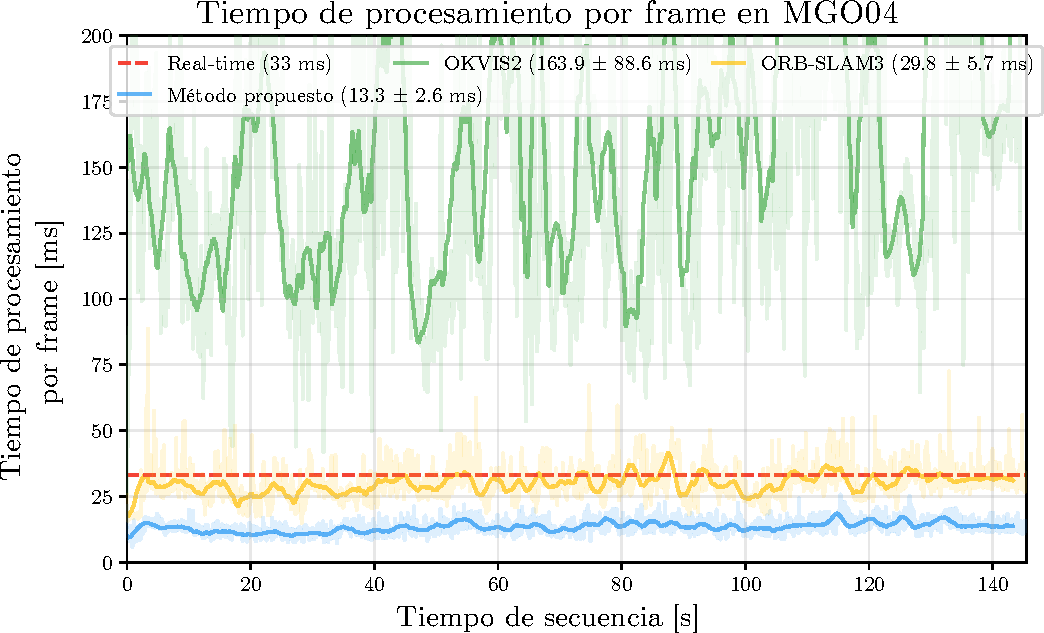
\includegraphics[width=1\linewidth]{images/MGO04.timings.sp.pdf}
    \caption{Tiempo de procesamiento por frame para cada sistema en la secuencia MGO04 del MSD, que cuenta con cuatro cámaras, en un procesador Intel Core Ultra 9 285H con 32 GB de RAM. Se muestra un promedio móvil con una ventana de 2 segundos (60 frames). En el fondo, los datos sin procesar muestran outliers y jitter para cada sistema. Una línea roja marca el límite de tiempo para la operación en tiempo real. Notar que ORB-SLAM3 procesa solo dos de las cuatro cámaras disponibles.}
    \label{fig:mgo04_frame_timings}
\end{figure}

La Figura~\ref{fig:msd_rootba_times} muestra los tiempos de ejecución de la optimización
global con la adaptación de RootBA en precisión simple y doble para los mapas globales de las secuencias del MSD. La precisión simple reduce la mediana del tiempo de optimización en un 50\% en MSD y EuRoC, y en un
42\% en TUM-VI, sin degradar la precisión de la estimación de trayectoria.

\begin{figure}[!htbp]
    \centering
    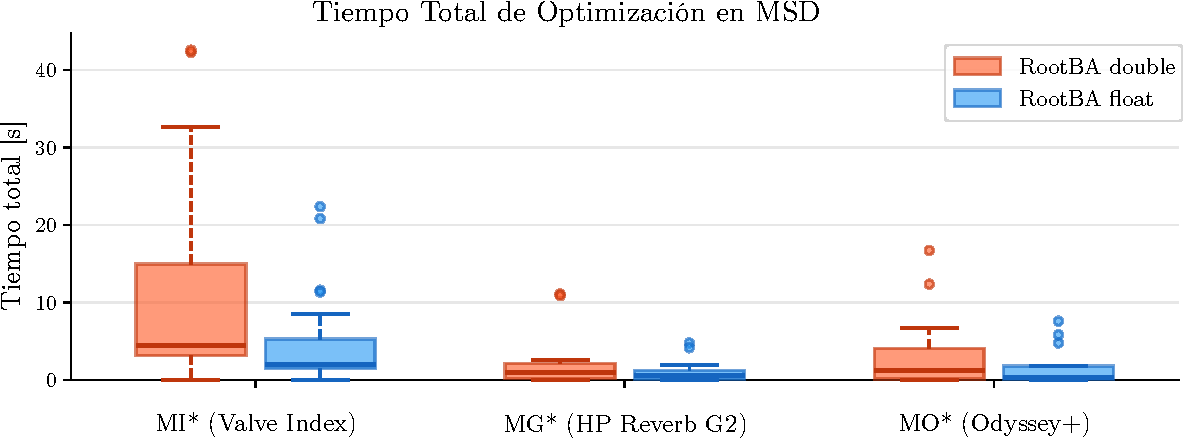
\includegraphics[width=1\linewidth]{images/msd.rootba.times.sp.pdf}
    \caption{Boxplots de tiempos totales de ejecución de la adaptación de RootBA en precisión simple y doble para cada tipo de secuencia del MSD. Ambas versiones fueron ejecutadas sobre el mismo mapa.}
    \label{fig:msd_rootba_times}
\end{figure}
